\documentclass[a4paper,12pt]{article}

\usepackage{graphicx}
\usepackage{caption}
\usepackage{subcaption}
\usepackage[utf8]{inputenc}
\usepackage[english,greek]{babel}
\usepackage{hyperref}
\usepackage{amsmath}

\title{Τεχνικές Βελτιστοποίησης - Εργασία 3}
\author{Ρουσομάνης Γεώργιος (ΑΕΜ: 10703)}
\date{Δεκέμβριος 2024}

\begin{document}

\maketitle

\section*{Εισαγωγή}

Στόχος της συγκεκριμένης εργασίας είναι η ελαχιστοποίηση μίας μη γραμμικής συνάρτησης $f(x)$, η οποία υπόκειται σε
περιορισμούς της μορφής $\alpha_i \leq x_i \leq \beta_i$, με τη χρήση της μεθόδου μέγιστης καθόδου με προβολή. 
Η αντικειμενική συνάρτηση που θα μελετηθεί είναι η:
\[
f(x) = \frac{1}{3} x_1^2 + 3 x_2^2, \quad x = \begin{bmatrix} x_1 \\ x_2 \end{bmatrix}.
\]
Η γραφική παράσταση της συνάρτησης παρουσιάζεται στο Σχ.~\ref{fig:objective_function}. 

Τα αποτελέσματα της μεθόδου μέγιστης καθόδου με προβολή θα συγκριθούν με εκείνα της κλασικής μεθόδου μέγιστης καθόδου
χωρίς περιορισμούς. Η ανάλυση θα περιλαμβάνει την επίδραση του βήματος $\gamma_k$ στη σύγκλιση της κλασικής μεθόδου, 
ενώ τα αποτελέσματα της προσομοίωσης στον υπολογιστή θα επαληθευτούν με μαθηματική ανάλυση.

Για τη μέθοδο μέγιστης καθόδου με προβολή, θα εξεταστεί η επίδραση του βήματος $\gamma_k$, της παραμέτρου $s_k$, 
καθώς και του σημείου εκκίνησης στη σύγκλιση της μεθόδου. 

\begin{figure}
    \centering
    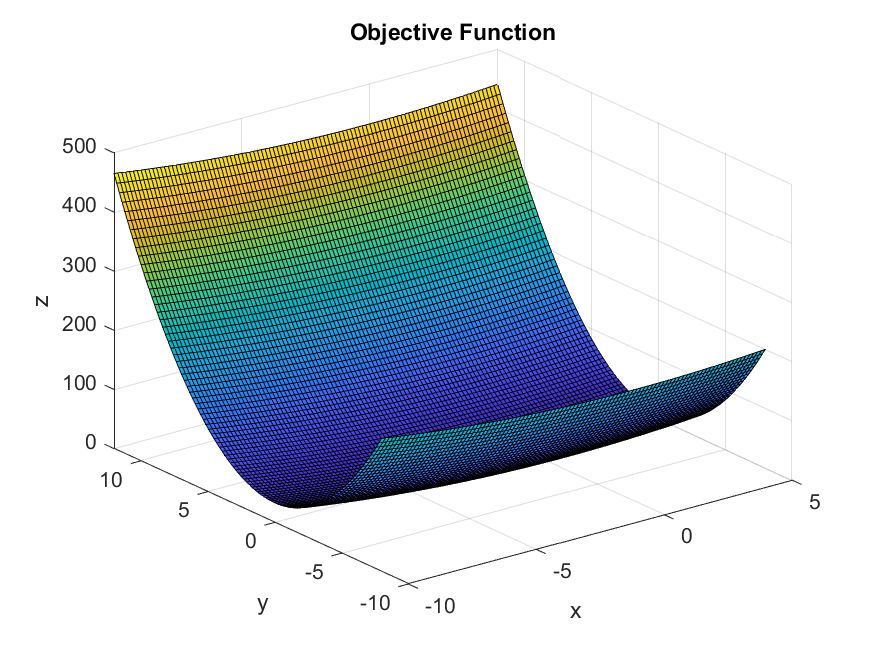
\includegraphics[width=1\linewidth]{plot/objective_function.pdf}
    \caption{Αντικειμενική Συνάρτηση}
    \label{fig:objective_function}
\end{figure}

\section*{Θέμα 1}
Όπως είναι ήδη γνωστό, η μέθοδος μέγιστης καθόδου αποτελεί μια τεχνική βελτιστοποίησης για προβλήματα απουσία 
περιορισμών. Ο αλγόριθμος υπολογίζει διαδοχικά σημεία μέσω της αναδρομικής σχέσης: 
\[
x_{k+1} = x_k - \gamma_k \nabla f(x_k) \implies 
\begin{bmatrix} x_{1(k+1)} \\ x_{2(k+2)} \end{bmatrix} = 
\begin{bmatrix} x_{1k} \\ x_{2k} \end{bmatrix}
 - \begin{bmatrix} \frac{2}{3} x_{1k} \\ 6 x_{2k} \end{bmatrix}
\]

Προφανώς, η $f$ παρουσιάζει ολικό ελάχιστο στο $x^* = (0,0)$. Για να συγκλίνει η μέθοδος για οποιοδήποτε αρχικό
σημείο $x_0 \neq x^*$ θα πρέπει να ισχύει:
\[
\left|\frac{x_{1(k+1)}}{x_{1k}}\right| < 1 \implies \left|1 - \frac{2}{3} \gamma_k \right| < 1 
\implies 0 < \gamma_k < 3
\]
και
\[
\left|\frac{x_{2(k+1)}}{x_{2k}}\right| < 1 \implies \left|1 - 6 \gamma_k \right| < 1 
\implies 0 < \gamma_k < \frac{1}{3}
\]
Από τα παραπάνω προκύπτει ότι για να έχουμε σύγκλιση στο $x^* = (0,0)$ θα πρέπει να ισχύει $0 < \gamma_k < \frac{1}{3}$.

Στο Σχ.~\ref{fig:task1_plot2} παρουσιάζεται το γράφημα σύγκλισης της αντικειμενικής συνάρτησης ως προς τον αριθμό των 
επαναλήψεων με αρχικό σημείο $x_0 = (5, -5)$, για διάφορες τιμές του $\gamma_k$. Παρατηρούμε ότι για $\gamma_k = 0.1$ 
και $\gamma_k = 0.3$ έχουμε επιτυχή σύγκλιση (δεδομένου ότι $\gamma_k < 1/3$), ενώ για $\gamma_k = 3$ και $\gamma_k = 5$
η μέθοδος αποκλίνει (δεδομένου ότι $\gamma_k > 1/3$). Το αποτέλεσμα αυτό συμφωνεί με τα συμπεράσματα της θεωρητικής 
ανάλυσης.

\begin{figure}[h]
    \centering
    \begin{minipage}{0.47\textwidth}
        \centering
        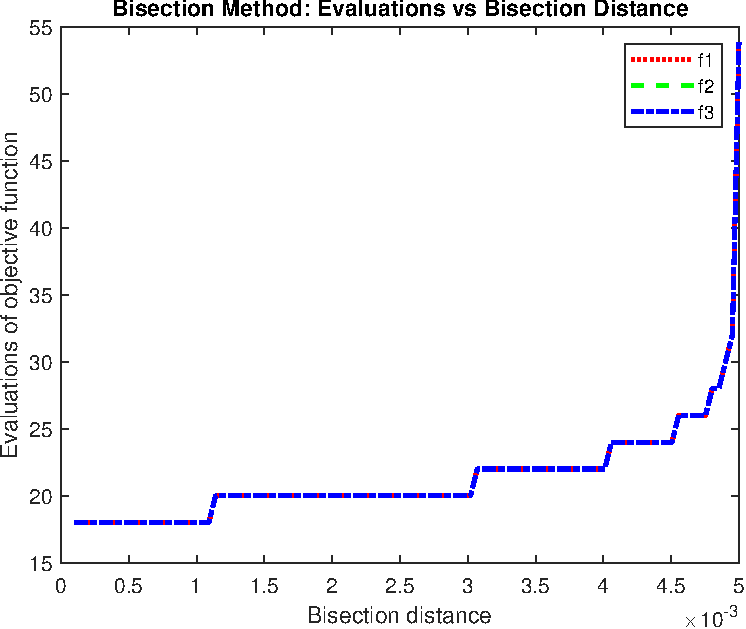
\includegraphics[width=1\linewidth]{plot/task1_plot1.pdf}
        \caption{\small Διαδοχικά σημεία υπολογισμού για το Θέμα 1}
        \label{fig:task1_plot1}
    \end{minipage} \hfill
    \begin{minipage}{0.47\textwidth}
        \centering
        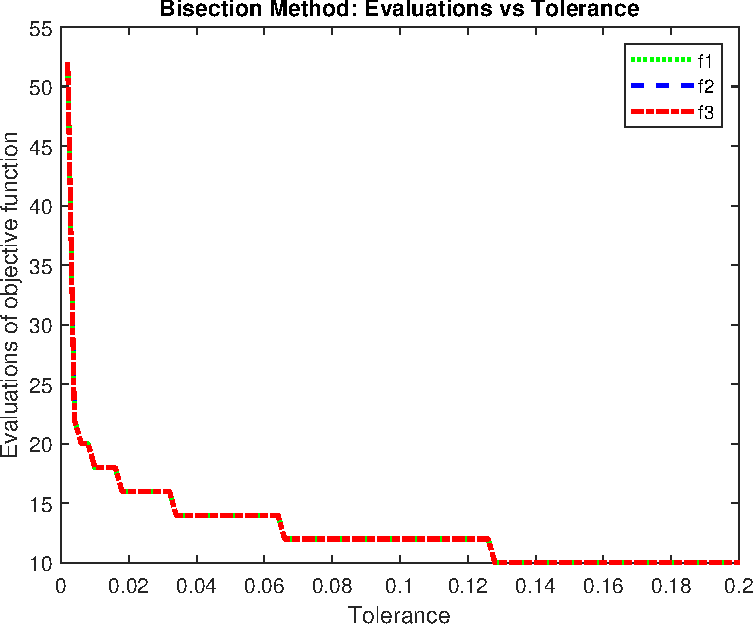
\includegraphics[width=1\linewidth]{plot/task1_plot2.pdf}
        \caption{\small Σύγκλιση της αντικειμενικής συνάρτησης ως προς τον αριθμό των επαναλήψεων για την μέθοδο μέγιστης καθόδου}
        \label{fig:task1_plot2}
    \end{minipage}
\end{figure}


\section*{Θέμα 2}
Η μέθοδος μέγιστης καθόδου με προβολή αποτελλεί μία τεχνική βελτιστοποίησης για προβλήματα με περιορισμούς.
Ο αλγόριθμος υπολογίζει διαδοχικά εφικτά σημεία της μορφής
\[
x_{k+1} = x_k + \gamma_k (\bar{x}_k - x_k), \quad \gamma_k \in (0, 1]
\]
όπου
\[
\bar{x}_k = Pr_X\{x_k - s_k \nabla f(x_k)\}, \quad s_k > 0.
\]
Επομένως, το $\bar{x}_k$ προσδιορίζεται από το $x_k$ αν κινηθούμε στην κατεύθυνση της αρνητικής κλήσης με
βήμα $s_k$ και στην συνέχεια βρούμε την προβολή του $x_k - s_k \nabla f(x_k)$ στο $X$, καταλήγοντας με τον
τρόπο αυτό σε εφικτό σημείο. Έχοντας βρει την εφικτή κατεύθυνση αναζήτησης $\bar{x}_k - x_k$, κινούμαστε με
βήμα $\gamma_k \in (0, 1]$ σ' αυτήν και προσδιορίζουμε το νέο εφικτό σημείο $x_{k+1}$.

Στο Σχ.~\ref{fig:task2_plot1} φαίνονται τα διαδοχικά σημεία που υπολογίζει ο αλγόριθμος μέγιστης καθόδου με
προβολή με σημείο αφετηρίας $x_0 = (5, -5)$ και $s_k = 5$, $\gamma_k = 0.5$.

\begin{figure}[h]
    \centering
    \begin{minipage}{0.47\textwidth}
        \centering
        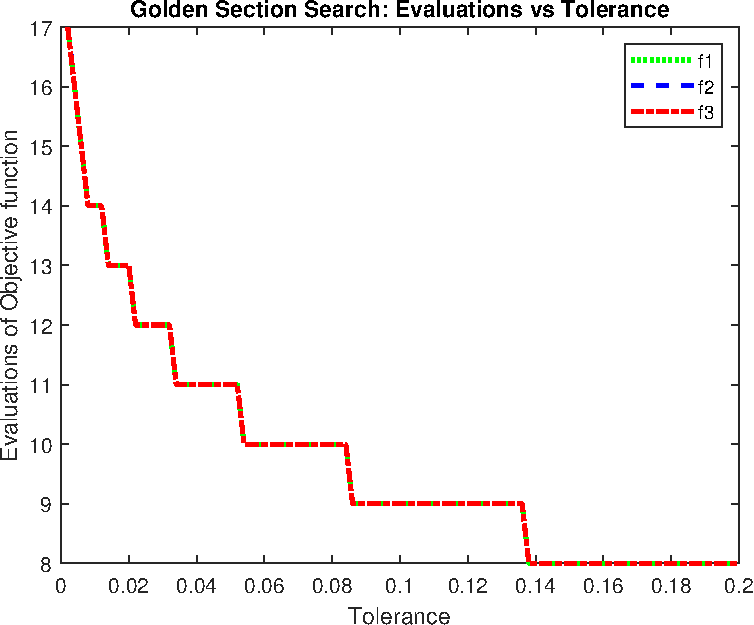
\includegraphics[width=1\linewidth]{plot/task2_plot1.pdf}
        \caption{\small Διαδοχικά σημεία υπολογισμού για το Θέμα 2}
        \label{fig:task2_plot1}
    \end{minipage} \hfill
    \begin{minipage}{0.47\textwidth}
        \centering
        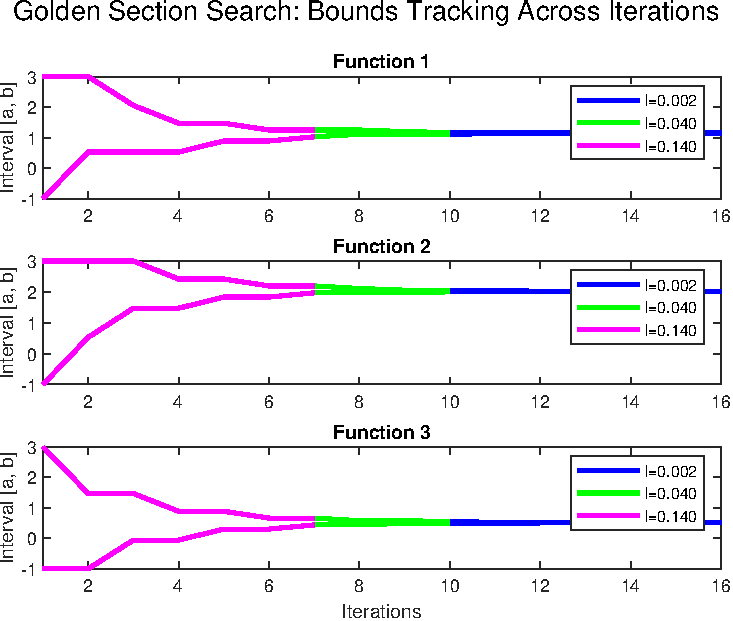
\includegraphics[width=1\linewidth]{plot/task2_plot2.pdf}
        \caption{\small Σύγκλιση της αντικειμενικής συνάρτησης ως προς τον αριθμό των επαναλήψεων για την μέθοδο μέγιστης καθόδου με προβολή}
        \label{fig:task2_plot2}
    \end{minipage}
\end{figure}

\section*{Συμπέρασμα}

\end{document}
